%% Preambulo, paquetes a cargar por compilador latex
\documentclass[12pt]{beamer}
\mode<presentation>{
  % selección de tema y color
  \usetheme{Copenhagen}
  \usecolortheme{orchid}
}

\usepackage[utf8]{inputenc}
\usepackage[spanish]{babel}
\usepackage{float}
\usepackage{graphicx}
\usepackage[font=scriptsize,labelfont=bf]{caption}
\usepackage{verbatim}
\usepackage{url} 
\usepackage[export]{adjustbox}
\usepackage{listings}
\usepackage{tcolorbox}
\usepackage{tikz}
\usepackage{cclicenses}
\usepackage{multicol}
\usepackage{ulem}
\newcommand{\soutthick}[1]{%
  \renewcommand{\ULthickness}{1.8pt}%
    \sout{#1}%
  \renewcommand{\ULthickness}{.4pt}% Resetting to ulem default
}
\usepackage[autostyle]{csquotes}
\lstdefinestyle{mystyle}{
  basicstyle=\tiny,
  language=Python
}
\lstset{style=mystyle}

%% Automatizar localización de las imágenes
\graphicspath{{../img/}}

\title{Qué es un programador ágil}
\author[Pepe Doval]{Pepe Doval}
\institute[SetPay | Agile Galicia]{SetPay | Agile Galicia}
\date{\today}

\begin{document}

\begin{frame}
  \titlepage
  \begin{tcolorbox}[]
    \centering
    {\small \bysa}\\
    {\tiny Esta obra está suxeita á licencia
      Recoñecemento-CompartirIgual 4.0 Internacional de Creative
      Commons. Para ver unha copia desta licencia, visite
      http://creativecommons.org/licenses/by-sa/4.0/.}
  \end{tcolorbox}
\end{frame}

\usebackgroundtemplate{%
  \tikz[overlay,remember picture] 
  \node[opacity=0.3 , at=(current page.south east),anchor=south east] {
    
\includegraphics[]{fondo}};
}


\title[Agile]{Agile}
\date{}
\author[Pepe Doval]{}
\institute{}

\section{Agile}
\label{sec:Agile}

\usebackgroundtemplate{}
\begin{frame}
  \titlepage
\end{frame}

\usebackgroundtemplate{%
  \tikz[overlay,remember picture] 
  \node[opacity=0.3 , at=(current page.south east),anchor=south east] {
    
\includegraphics[]{fondo}};
}

\subsection{Agile}
\label{subsec:Agile}

\begin{frame}
  \frametitle{El programador ágil}
  \begin{figure}[ht]
    
\includegraphics[scale=0.4]{zen_developer}
    \caption{https://www.apico.net/blog/how-bad-software-developer-are-you.html}
  \end{figure}
\end{frame}

\begin{frame}
  \frametitle{El programador frágil}
  \begin{figure}[ht]
    
\includegraphics[scale=0.4]{happy_monkey}
    \caption{https://www.apico.net/blog/how-bad-software-developer-are-you.html}
  \end{figure}
\end{frame}

\begin{frame}
  \frametitle{El plan}
  \begin{figure}[ht]
    
\includegraphics[scale=0.1]{plan}
    \caption{https://pixabay.com/p-618371/}
  \end{figure}
\end{frame}

\begin{frame}
  \frametitle{Cuando los planes salen bien}
  \begin{figure}[ht]
    
\includegraphics[scale=0.6]{successful_plan}
  \end{figure}
\end{frame}

\begin{frame}
  \frametitle{Metáfora del cañón}
  \begin{figure}[ht]
    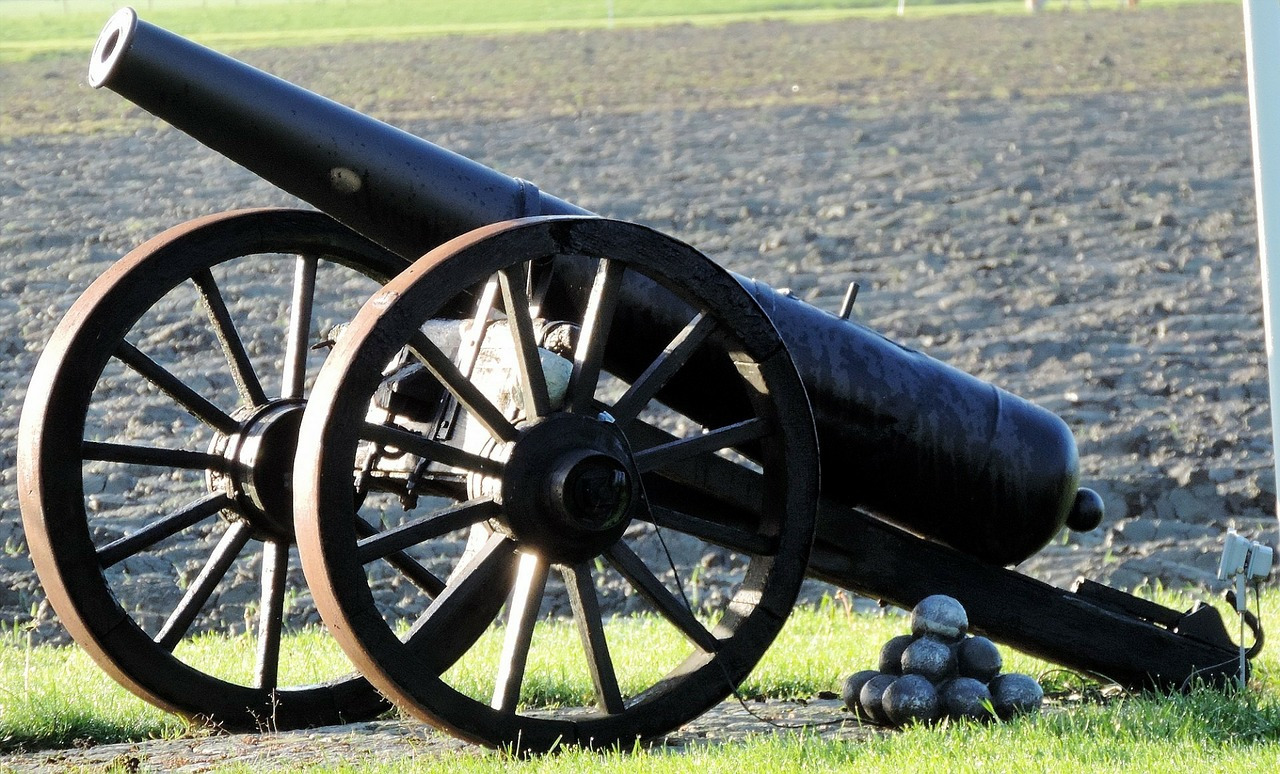
\includegraphics[scale=0.2]{cannon}
    \caption{http://maxpixel.freegreatpicture.com/Cannonballs-Weapon-Cannon-Cannonball-History-War-314498}
  \end{figure}
\end{frame}

\begin{frame}
  \frametitle{Asunciones del programador frágil}
  \begin{itemize}
  \item El cliente \textbf{sabe} lo que quiere
  \item El programador(equipo) \textbf{sabe} cómo construirlo
  \item \textbf{No} ocurren cambios durante el desarrollo
  \end{itemize}
\end{frame}

\begin{frame}
  \frametitle{Asunciones del programador ágil}
  \begin{itemize}
  \item El cliente \textbf{\soutthick{sabe} descubre} lo que quiere
  \item El programador(equipo) \textbf{\soutthick{sabe} descubre} cómo construirlo
  \item \textbf{\soutthick{No}} ocurren cambios durante el desarrollo
  \end{itemize}
\end{frame}

\begin{frame}
  \frametitle{Manifesto}
  \begin{figure}[ht]
    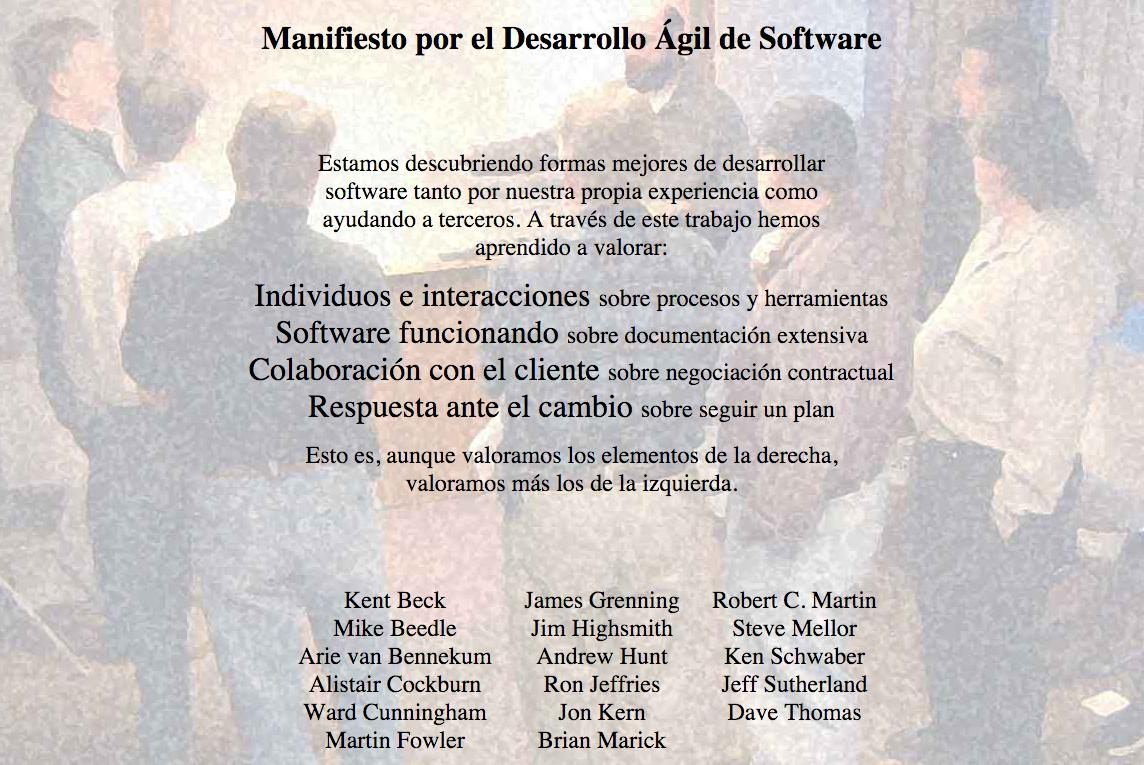
\includegraphics[scale=0.2]{manifesto}
    \caption{http://agilemanifesto.org/}
  \end{figure}
\end{frame}
               % introducción a agile
% !TeX spellcheck = es_ES

\title[Prácticas ágiles]{Prácticas}
\date{}
\author[Pepe Doval]{}
\institute{}

\section{Prácticas}
\label{sec:Practicas}

\usebackgroundtemplate{%
  \tikz[overlay,remember picture] 
  \node[opacity=0.3 , at=(current page.south east),anchor=south east] {
    
\includegraphics[]{fondo}};
}

\begin{frame}
  \titlepage
  \begin{figure}[ht]
    \centering
    \vspace*{-2.5cm}
  \end{figure}
\end{frame}

\subsection{Prácticas habituales}
\label{subsec:Practicas}

\begin{frame}
  \frametitle{Al programar (1/2)}
  \begin{itemize}
    \item Pair programming
    \item TDD
    \item Refactorización
    \item Integración continua
  \end{itemize}
\end{frame}

\begin{frame}
  \frametitle{Al programar (2/2)}
  \begin{itemize}
    \item Diseño simple
    \item Propiedad colectiva del código
    \item Estándares y convenciones
  \end{itemize}
\end{frame}

\begin{frame}
  \frametitle{Al planificar (1/2)}
  \begin{itemize}
    \item Iteraciones
    \item Time boxing
    \item Planning game
    \item Standup meetings
  \end{itemize}
\end{frame}

\begin{frame}
  \frametitle{Al planificar (2/2)}
  \begin{itemize}
    \item Automatización
    \item Radiadores de información
    \item Definitions of done
  \end{itemize}
\end{frame}

\begin{frame}
  \frametitle{Al aprender (1/2)}
  \begin{itemize}
    \item Katas
    \item Coding Dojos
    \item Mob programming
    \item Desksurfing
  \end{itemize}
\end{frame}

\begin{frame}
  \frametitle{Al aprender (2/2)}
  \begin{itemize}
    \item Patrones de aprendizaje
    \item Mentoring
    \item Artesanía del software
  \end{itemize}
\end{frame}

\begin{frame}
  \frametitle{El ingrediente secreto}
  \begin{figure}[ht]
    \centering
    
\includegraphics[scale=0.15]{ingrediente_secreto}
    \caption{http://kungfupanda.wikia.com/}
  \end{figure}
\end{frame}

\begin{frame}
  \frametitle{Agile}
  \begin{figure}[ht]
    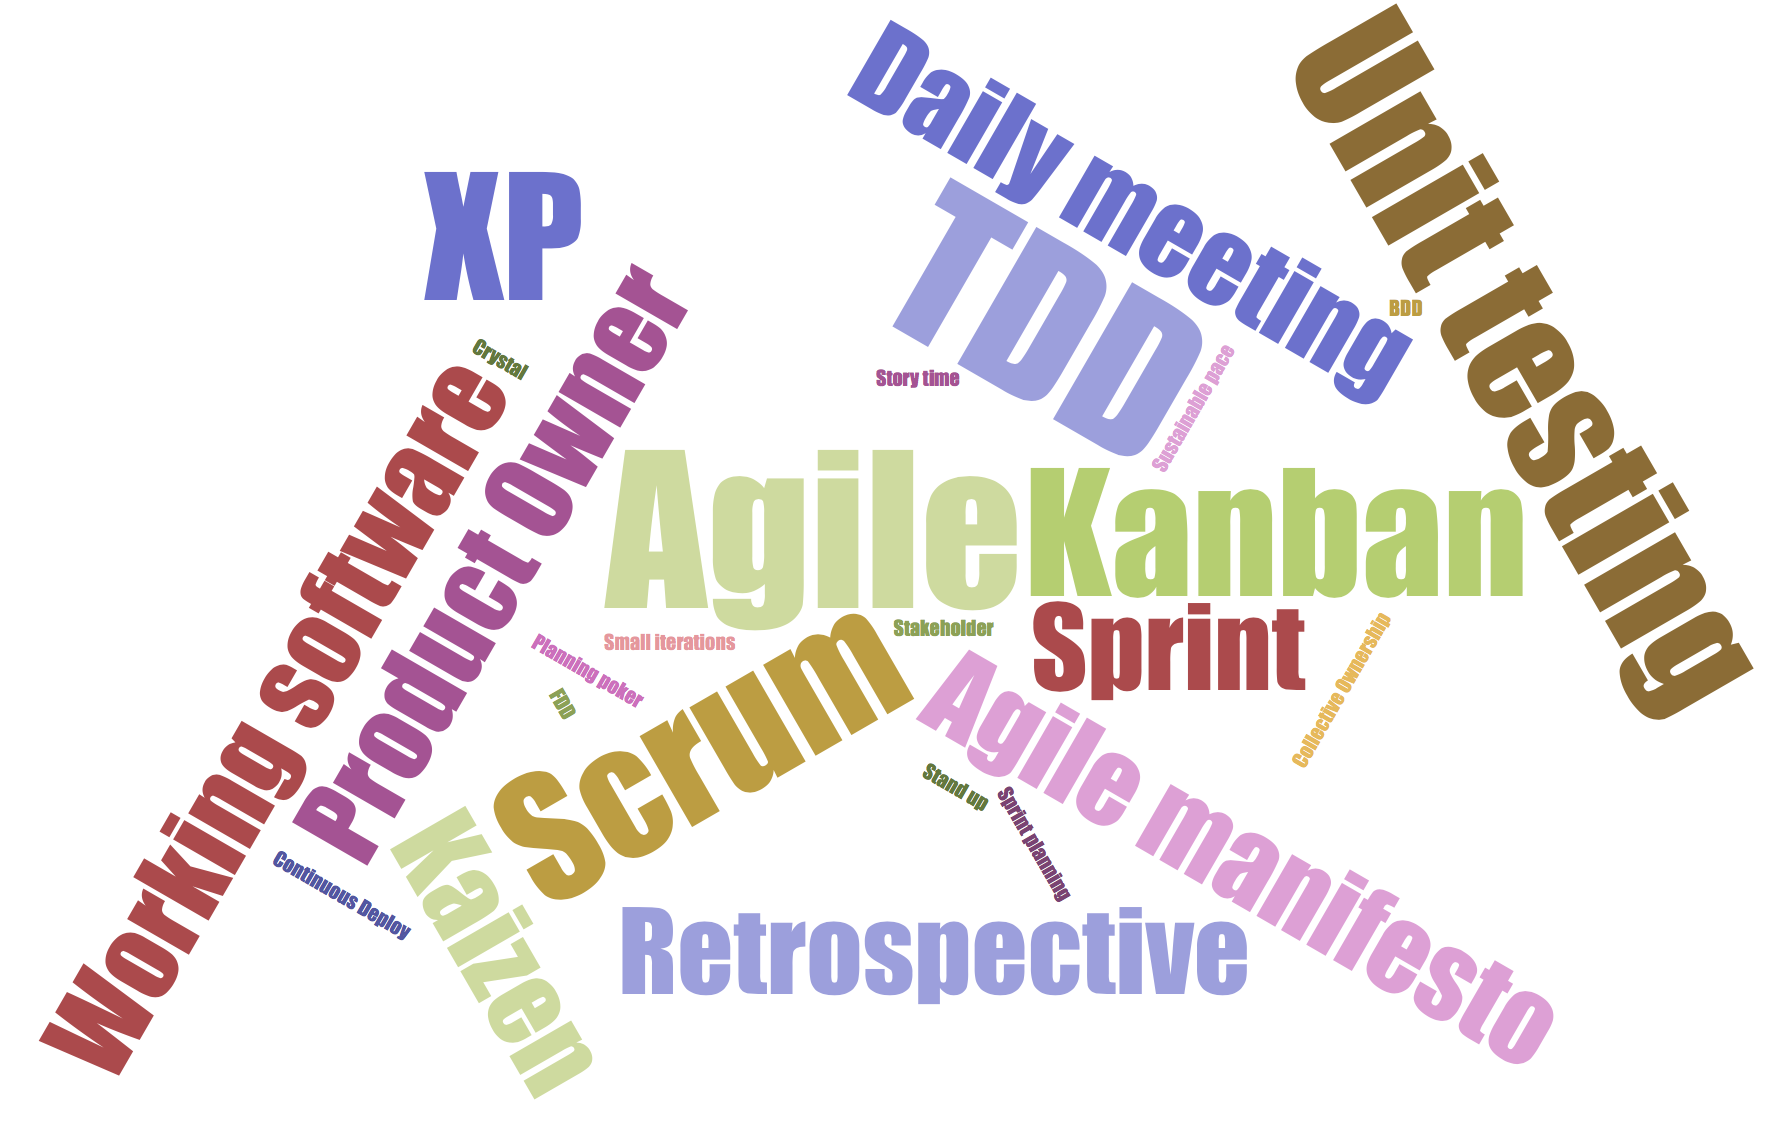
\includegraphics[scale=0.3]{cloud_agile}
  \end{figure}
\end{frame}
                 % prácticas del programador ágil

\end{document}
